\def\SECTION{1.2 Segment Addition Postulate}
\documentclass[aspectratio=169,14pt]{beamer}
\usepackage[T1]{fontenc}
\usepackage{mathpazo}
\usepackage{amsmath,amssymb}
\usepackage{tikz}
\usetikzlibrary{arrows.meta,calc,decorations.pathreplacing}
\definecolor{fblue}{HTML}{1F4E79}
\definecolor{fteal}{HTML}{0F7C7C}
\definecolor{fgold}{HTML}{C9962B}
\definecolor{fred}{HTML}{B3261E}
\definecolor{fink}{HTML}{16233B}
\definecolor{fsoft}{HTML}{EEF3F8}
\definecolor{fgoldsoft}{HTML}{FBF1DC}
\setbeamertemplate{navigation symbols}{}
\setbeamercolor{normal text}{fg=fink}
\setbeamercolor{frametitle}{fg=fblue}
\setbeamerfont{frametitle}{series=\bfseries,size=\Large}
\setbeamercolor{structure}{fg=fteal}
\setbeamertemplate{itemize item}{\color{fteal}$\blacktriangleright$}
\setbeamertemplate{frametitle}{\vspace{6pt}\insertframetitle\par\vspace{-2pt}{\color{fgold}\rule{2.2cm}{2pt}}}
\setbeamertemplate{footline}{\hspace{0.6cm}{\color{fblue}\scriptsize\bfseries Fang\textcolor{fteal}{Math}}\hfill{\scriptsize\color{gray}\SECTION\quad\insertframenumber}\hspace{0.6cm}\vspace{6pt}}
\newcommand{\key}[1]{{\color{fteal}\textbf{#1}}}
\newcommand{\ans}[1]{\colorbox{fgoldsoft}{\color{fink}\ensuremath{#1}}}
\newcommand{\warn}[1]{\begin{beamercolorbox}[sep=8pt,rounded=true]{warnbox}{\color{fred}\textbf{Watch out!}}\enskip #1\end{beamercolorbox}}
\setbeamercolor{warnbox}{bg=fred!8,fg=fink}
\setbeamercolor{turnbox}{bg=fgoldsoft,fg=fink}
\setbeamercolor{defbox}{bg=fsoft,fg=fink}
\newcommand{\defn}[1]{\begin{beamercolorbox}[sep=8pt,rounded=true]{defbox}#1\end{beamercolorbox}}
\newenvironment{yourturn}{\begin{beamercolorbox}[sep=10pt,rounded=true]{turnbox}{\color{fgold}\Large\bfseries Your turn!}\quad{\small Pause the video and try it.}\par\medskip}{\end{beamercolorbox}}
\newcommand{\titleframe}[3]{%
\begin{frame}[plain]
\begin{tikzpicture}[remember picture,overlay]
\fill[fblue] (current page.north west) rectangle ([yshift=-0.9cm]current page.north east);
\node[anchor=west,text=white,font=\bfseries] at ([xshift=0.6cm,yshift=-0.45cm]current page.north west) {Fang\textcolor{fgold}{Math}};
\node[anchor=east,text=white,font=\small] at ([xshift=-0.6cm,yshift=-0.45cm]current page.north east) {Geometry $\cdot$ Chapter 1};
\end{tikzpicture}
\vfill
{\color{fteal}\large\bfseries #1}\par\medskip
{\color{fblue}\fontsize{30}{34}\selectfont\bfseries #2}\par\medskip
{\color{fgold}\rule{3cm}{3pt}}\par\bigskip
{\large #3}
\vfill
{\small\color{gray} fangmath.com $\cdot$ YouTube @fangmathcom}
\end{frame}}
\newcommand{\closeframe}[1]{%
\begin{frame}{Remember}
#1
\vfill
\begin{center}{\color{fblue}\large\bfseries Now practice at your level:}\par\smallskip
{\Large\color{fteal}\bfseries fangmath.com} \enskip{\color{gray}$\to$ Geometry $\to$ Chapter 1}\end{center}
\end{frame}}

\begin{document}
\titleframe{Lesson 1.2}{Segment Addition Postulate}{Part $+$ part $=$ whole}

\begin{frame}{Walk 4 steps, then 7 more}
\centering
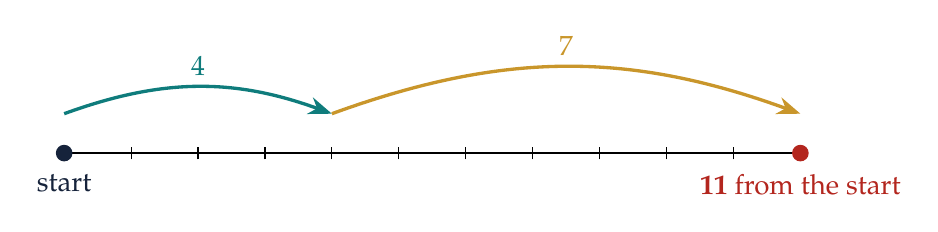
\begin{tikzpicture}[x=0.85cm]
\draw[thick] (0,0)--(11,0);
\foreach \i in {0,...,11} \draw (\i,-0.08)--(\i,0.08);
\fill[fink] (0,0) circle(3pt) node[below=4pt]{start};
\onslide<2->{\draw[fteal,very thick,-{Stealth}] (0,0.5) to[bend left=20] node[above]{$4$} (4,0.5);}
\onslide<3->{\draw[fgold,very thick,-{Stealth}] (4,0.5) to[bend left=20] node[above]{$7$} (11,0.5);}
\onslide<4->{\fill[fred] (11,0) circle(3pt) node[below=4pt]{\textbf{11} from the start};}
\end{tikzpicture}
\par\bigskip
\onslide<4->{\Large $4 + 7 = 11$ \quad {\normalsize --- you just used today's postulate.}}
\end{frame}

\begin{frame}{The postulate}
\centering
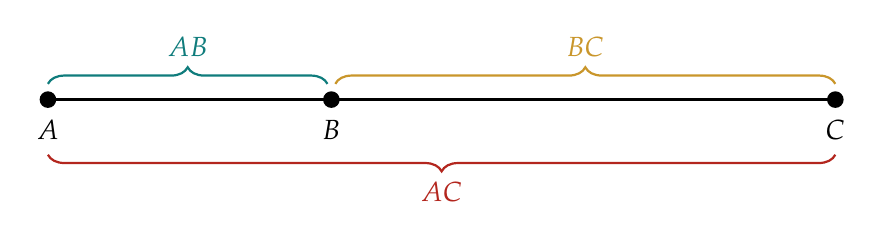
\begin{tikzpicture}[x=1cm]
\draw[very thick] (0,0)--(10,0);
\fill (0,0) circle(3pt) node[below=4pt]{$A$} (3.6,0) circle(3pt) node[below=4pt]{$B$} (10,0) circle(3pt) node[below=4pt]{$C$};
\onslide<2->{\draw[fteal,thick,decorate,decoration={brace,amplitude=6pt}] (0,0.2)--(3.55,0.2) node[midway,above=6pt]{$AB$};
\draw[fgold,thick,decorate,decoration={brace,amplitude=6pt}] (3.65,0.2)--(10,0.2) node[midway,above=6pt]{$BC$};}
\onslide<3->{\draw[fred,thick,decorate,decoration={brace,amplitude=6pt,mirror}] (0,-0.7)--(10,-0.7) node[midway,below=6pt]{$AC$};}
\end{tikzpicture}
\par\bigskip
\onslide<4->{\defn{\centering If $B$ is \key{between} $A$ and $C$, then \quad {\Large $AB + BC = AC$}}}
\end{frame}

\begin{frame}{Simple cases first}
\begin{columns}[T]
\begin{column}{0.48\textwidth}
\key{Find the whole: add}\par\medskip
$AB = 4,\ BC = 7$\par\smallskip
\pause $AC = AB + BC$\par\smallskip
\pause $AC = 4 + 7 = \ans{11}$
\end{column}
\begin{column}{0.48\textwidth}
\pause
\key{Know the whole and one piece: subtract}\par\medskip
$AC = 20,\ AB = 8$\par\smallskip
\pause $BC = AC - AB$\par\smallskip
\pause $BC = 20 - 8 = \ans{12}$
\end{column}
\end{columns}
\end{frame}

\begin{frame}{With algebra}
$AB = x + 3,\quad BC = 2x,\quad AC = 21.$ \quad Find $x$ and $BC$.\par\bigskip
\begin{tabular}{l l}
\onslide<2->{$(x + 3) + 2x = 21$} & \onslide<2->{\small\color{gray} part $+$ part $=$ whole}\\[6pt]
\onslide<3->{$3x + 3 = 21$} & \onslide<3->{\small\color{gray} combine like terms}\\[6pt]
\onslide<4->{$3x = 18$} & \onslide<4->{\small\color{gray} subtract 3}\\[6pt]
\onslide<5->{$x = 6$} & \onslide<5->{\small\color{fred}\textbf{don't stop at $x$!}}\\[6pt]
\onslide<6->{$BC = 2(6) = \ans{12}$} & \onslide<6->{\small\color{gray} the question asked for $BC$}\\[6pt]
\onslide<7->{Check: $AB = 9$,\ $9 + 12 = 21$ \checkmark} & \\
\end{tabular}
\end{frame}

\begin{frame}{Only when $B$ is between $A$ and $C$}
\begin{columns}[c]
\begin{column}{0.45\textwidth}\centering
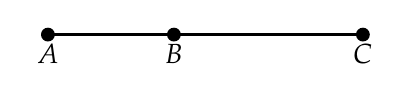
\begin{tikzpicture}
\draw[very thick] (0,0)--(4,0);
\fill (0,0) circle(2.5pt) node[below]{$A$} (1.6,0) circle(2.5pt) node[below]{$B$} (4,0) circle(2.5pt) node[below]{$C$};
\end{tikzpicture}\par\medskip
{\color{fteal}\checkmark} $AB + BC = AC$
\end{column}
\begin{column}{0.45\textwidth}\centering
\pause
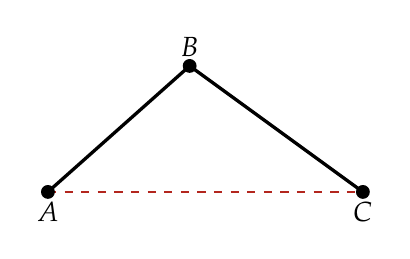
\begin{tikzpicture}
\draw[very thick] (0,0)--(1.8,1.6)--(4,0);\draw[thick,dashed,fred] (0,0)--(4,0);
\fill (0,0) circle(2.5pt) node[below]{$A$} (1.8,1.6) circle(2.5pt) node[above]{$B$} (4,0) circle(2.5pt) node[below]{$C$};
\end{tikzpicture}\par\medskip
{\color{fred}$\times$} $AB + BC > AC$
\end{column}
\end{columns}
\bigskip\pause
\warn{If $A$, $B$, $C$ make a triangle, the two sides add up to \textbf{more} than $AC$.}
\end{frame}

\begin{frame}{}
\begin{yourturn}
$Q$ is between $P$ and $R$.\quad $PQ = 3x - 1,\quad QR = x + 5,\quad PR = 24.$\par\medskip
Find $x$ and $PQ$.
\end{yourturn}
\pause\bigskip
$(3x - 1) + (x + 5) = 24 \;\Rightarrow\; 4x + 4 = 24 \;\Rightarrow\; x = \ans{5}$\par\medskip
\pause $PQ = 3(5) - 1 = \ans{14}$ \qquad {\small\color{gray} check: $14 + 10 = 24$ \checkmark}
\end{frame}

\closeframe{\begin{itemize}\setlength\itemsep{10pt}
\item \key{Part $+$ part $=$ whole}: \ $AB + BC = AC$ when $B$ is between $A$ and $C$.
\item Missing piece? \key{Subtract} from the whole.
\item Solve for $x$ --- then answer the question they actually asked.
\end{itemize}}
\end{document}
